%%%%%%%%%%%%%%%%%%%%%%%%%%%%%%%%%%%%%%%%%%%%%
\section{Visual Encodings}
\label{sec:visual-encodings}
%%%%%%%%%%%%%%%%%%%%%%%%%%%%%%%%%%%%%%%%%%%%%

Pangea is composed of 3 primary visual components. Each component is
tailored to understading systems at different granulairities. The
first component is the time curve. The time curve plots a point for
each snapshot collected from a systems logs. The distance between each
point is the difference in their state as caclculated in
Section~\ref{differentiation-algorithm}. The points are connected by a
curve which links them temporally, creating an approximate FSM from
the exection. Second likely data invariants, mined from the logs, are
plotted graphically. Points in the graph are logged variables colleted
from all nodes present at runtime. Edges connecting the points are
invariants on their values. Finally Pangaea rendereds a ShiViz style
communication graph. The vertical lines of the graph correspond to
individual nodes. Edges between the vertical lines are messages sent
between the nodes. Together these visuals provide a comprehensive view
of the systems runtime behaviour.

To generate examples of our visualizations we insturmented and
exeucted a three node cluster of etcd~\cite{etcdraft}. Etcd is a
popular, and industrial scale raft implemntation. Raft is a fault
tolerant concuss algorithm. Etcd raft implements a key value store
which allows users to issue put and get requets. For the sake of
example our visualization were taken from a run in which a client
issued 50 put requests, followed by 50 get requests.

\subsection{Time Curve}


        Each point in the time curve correlates to a single snapshot.
        Therein each point is representative of the system as a whole.
        A result of calculating the differental of each snapshot, is
        that system states which are similar to one another are
        clustered togeher, while differing states are further apart.
        This clustering allows users to quickly associate similar
        states of their system. Each point is also color coded based
        on their temporal ordering. The first snapshot is colored
        bright red, and the final snapshot is dark brown. All
        intermediate points are colored as an intermediate hue. By
        coloring each of the points users can associate custered state
        with a time in the systems execution. The starting and end
        snapshots are significant because they orient the users
        reasoning about their system. Starting and end points are
        circled in blue to make them identifiable.

        All points in the graph are connected by a single curve. The
        curve begins at the starting point, ends at the end point, and
        connects all points sequentially as they occur in logical
        time. The curve is color coded identically with the points. It
        begins as bright red, and transitions to dark brown. Where the
        cuver intersects with a point their colors match. The purpose
        of color coding the time curve is to allow users to quickly
        associate a temporal relasionship on transitions between
        states. A legend which describes these encodings is positioned
        in the top right of the graph.

        Users interact with the curve by selecting an individual
        snapshot. When selected concrete information about the
        snapshot is provided to the user. First, the corresponding cut
        of the network from on which the snapshot was taken is
        highlighted on the process communication graph (see
        Section~\ref{communication-graph}). Second the user is
        presented with a table of variables and their values from the
        snapshot. The table contains information about the node a
        variable was resident on, the name of the variable, the
        variables type, and its value. Additionally a table containing
        the vector clocks on each node is rendered to help users
        identify the precise moment the snapshot was taken. Concrete
        values alow users to reason precicely about the state of the
        system. Users can invstigate which variable assignment
        correspond to clusters in the curve. In the cases of divergent
        or unexpected clustering users can associate concrete state
        with the behaviour of their system.

        In Figure~\ref{fig:put-get-curve} the bright red cluster, and
        brown cluster correspond to snapshots in which put, and get
        requests were being serviced respectivly. A single connection
        in the curve links the red cluster to the brown cluster and
        denots the transition from one distinct functionality to the
        next. A small cluster containing the inital snapshot is
        differentiated from the two main clusters. This small cluster
        corresponds to a leader election triggered at the beginning of
        the clusters execution.

\begin{figure}[h]
    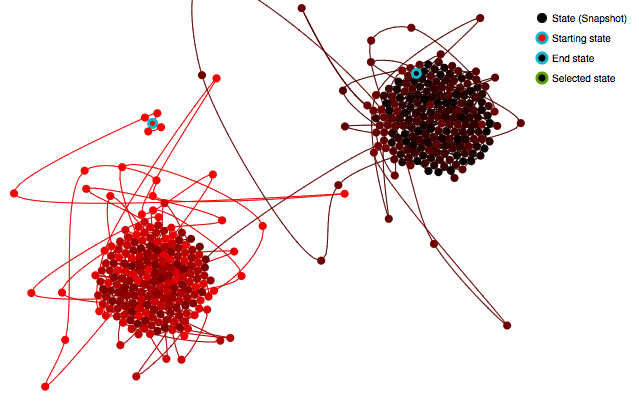
\includegraphics[width=\linewidth]{fig/put-get-curve}%
    \caption{Time curve generated from an etcd raft cluster processing 50 put requets, followed by 50 get requests.\label{fig:put-get-curve}}%
\end{figure}
    


\subsection{Invarinat Graph}
\label{invariant-graph}

\subsection{Communication Graph}
\label{communication-graph}

\begin{itemize}
    \item \textbf{Why visualization}
    \item \textbf{What components can be visualized}
    \item \textbf{How can visuals guide deveopers to identify deviant behaviour}
    \item \textbf{Choice of encodings}
    \item \textbf{Time Curve}
    \item \textbf{Invariants}
    \item \textbf{Time line}
    \item \textbf{Concrete Values}
\end{itemize}
